\chapter{Các thuật toán tìm kiếm}

%%%%
\section{Breadth-first Search (BFS)}

\subsection{Ý tưởng chính}

BFS hay \textit{tìm kiếm theo chiều rộng} sẽ tìm kiếm bằng cách tạo một \textit{cây tìm kiếm} thông qua không gian trạng thái (tức là biểu diễn bằng cây thay vì bằng đồ thị như ta nói phía trên). Thực hiện như nguyên lý tìm kiếm đồ thị ở hình \ref{fig:illu} và thuật toán \ref{algo:1}, nhưng lúc này ta xem \textit{frontier} như một hàng đợi, những nút nào vào trước sẽ được lấy ra trước. Do đó tại nút ở độ sâu $d$ của cây tìm kiếm, ta sẽ mở rộng tất cả các nút con của nó ở độ sâu $d+1$. Với cách này ta có thể đi đến mọi trạng thái của bài toán bằng cách mở rộng cây tìm kiếm, khiến cây tìm kiếm ngày càng ``rộng'' ra cho đến khi nào ta tìm được đích.

\subsection{Mã giả}

\begin{algorithm}[H]
  $start \gets \text{trạng thái bắt đầu}$\;
  \tcc{ta xem \textit{frontier} như là một hàng đợi}
  $frontier \gets \{start\}$\; 
  $expanded \gets \emptyset$\;
  $goal \gets \text{hàm xem nút hiện tại có là trạng thái đích hay chưa}$\;
  $T \gets \text{hàm chuyển trạng thái con}$\;
  \While{$frontier \neq \emptyset$}
  {
      $current \gets \text{nút được lấy ra từ $frontier$}$\;
      \text{Thêm $current$ vào $expanded$}\;
      \eIf{$goal(current)$}
      {
        \KwRet{\text{đã tìm thấy đáp án}}\;
      }{
        \For{$neighbor \in T(current)$}
        {
            \If{$neighbor \notin frontier$ và $neighbor \notin expanded$} 
            {
                \text{Thêm $neigbor$ vào $frontier$}\;
            }
        }
      }
  }
  \KwRet{\text{không tìm thấy đáp án}}\;
  \caption{Breadth-First-Search}
  \label{algo:BFS}
\end{algorithm}

\subsection{Ví dụ}

\begin{figure}[H]
    \centering
    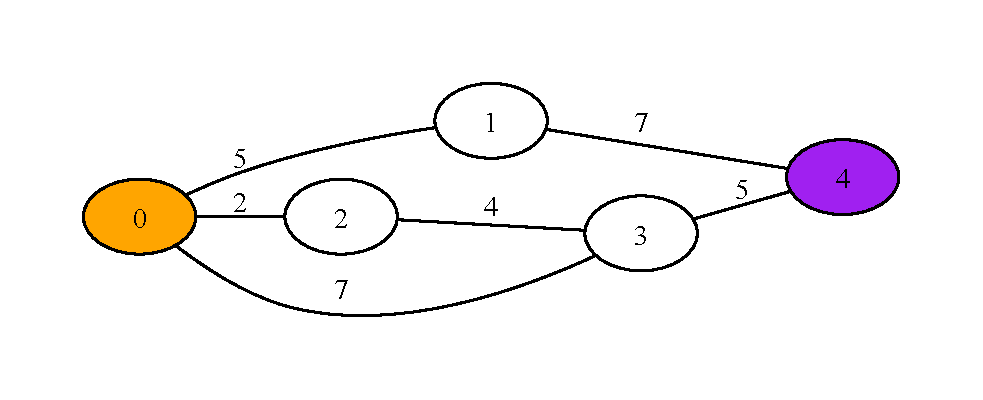
\includegraphics[scale=0.8]{figure/init.pdf}
    \caption{Ta sẽ dùng đồ thị như hình để thực hiện tìm kiếm, trong đó trạng thái bắt đầu có màu cam và trạng thái kết thúc có màu tím.}
    \label{fig:init}
\end{figure}

\begin{figure}[H]
    \centering
    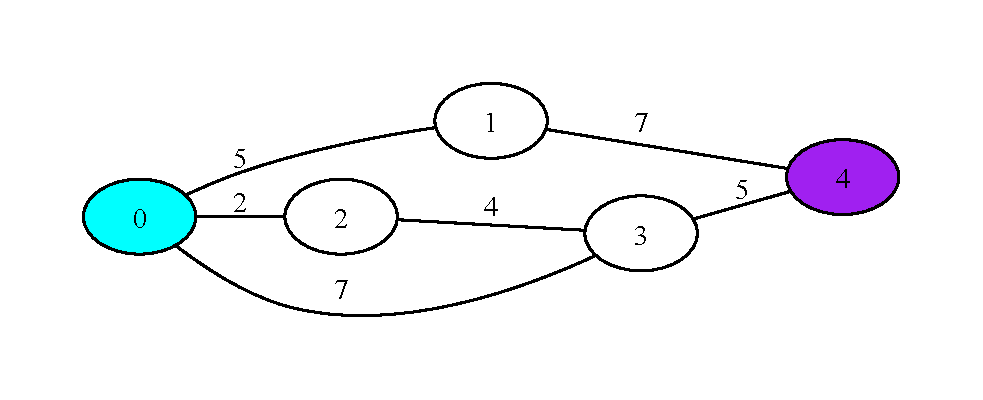
\includegraphics[scale=0.8]{figure/BFS/0.pdf}
    \caption{Đầu tiên, BFS xuất phát ở trạng thái bắt đầu và đưa nút đầu tiên vào \textit{frontier} (ta tô màu xanh cho các nút trong \textit{frontier}).}
    \label{fig:BFS_0}
\end{figure}

\begin{figure}[H]
    \centering
    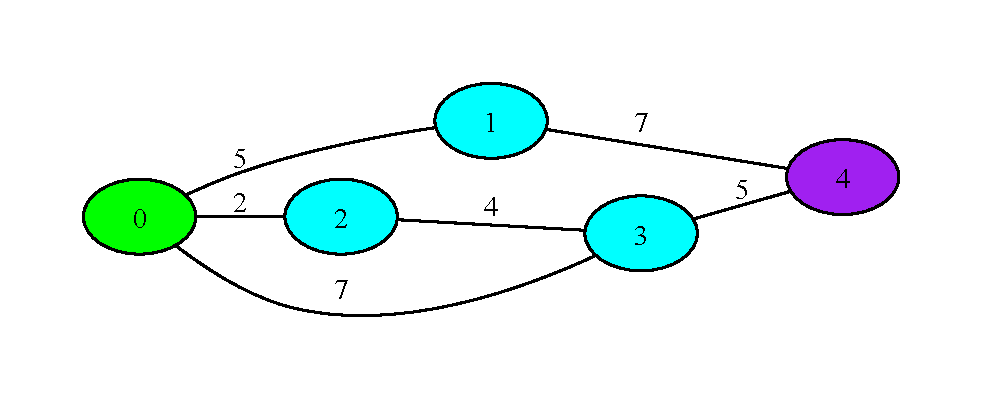
\includegraphics[scale=0.8]{figure/BFS/1.pdf}
    \caption{Tiếp theo BFS đưa nút hiện tại (là nút ban đầu) vào \textit{expanded} (ta tô màu xanh lá cây) và mở rộng các nút con, đưa các nút đó vào \textit{frontier}.}
    \label{fig:BFS_1}
\end{figure}

\begin{figure}[H]
    \centering
    \includegraphics[scale=0.7]{figure/BFS/2.pdf}
    \includegraphics[scale=0.7]{figure/BFS/3.pdf}
    \includegraphics[scale=0.7]{figure/BFS/4.pdf}
    \caption{Do \textit{frontier} là một hàng đợi nên tại BFS đã mở rộng hết tất cả các nút cùng chiều sâu (là $1$, $2$, $3$).}
    \label{fig:BFS_2_4}
\end{figure}

\begin{figure}[H]
    \centering
    \includegraphics[scale=0.8]{figure/BFS/5.pdf}
    \caption{Và cuối cùng BFS dừng khi nó đã đến (ta xem các nút ở \textit{frontier} như các nút ta đã thấy nhưng chưa được mở rộng và ta sẽ kiểm tra trạng thái đích ở các nút đã được mở rộng) được trạng thái đích (là $4$).}
    \label{fig:BFS_5}
\end{figure}

\subsection{Đánh giá}

\begin{itemize}
    \item \textbf{Tính đầy đủ}: dễ thấy, do BFS sẽ đi đến tất cả các trạng thái mà có thể đi được từ trạng thái ban đầu, do đó BFS có tính hệ thống, vậy BFS có tính đầy đủ. Nhưng lưu ý rằng, chỉ có tính đầy đủ khi và chỉ khi hệ số phân nhánh tiến của một nút bất kì là hữu hạn, bởi vì nếu vô hạn thì ở độ sâu $d+1$ của nút có độ sâu $d$ sẽ có vô hạn nút, do đó BFS sẽ mất vô hạn thời gian để mở rộng các nút đó.

    \item \textbf{Tính tối ưu}: Trong trường hợp đồ thị có chi phí là bằng nhau từ trạng thái bắt đầu đến một độ sâu $d$ bất kì, khi đó BFS sẽ có tính tối ưu do nó tìm được đáp án có ``chi phí'' ít nhất, chi phí ở đây là số nút mà nó phải đi qua. Thế nhưng trong các đồ thị có chi phí ví dụ như trọng số, thì số nút ngắn nhất không có nghĩa là chi phí ít nhất, do đó không thoả mãn tính tối ưu.

    \item \textbf{Độ phức tạp thời gian}: Giả sử rằng ở một độ sâu bất kì, nút có hệ số phân nhánh tiến là $b$ và giả sử đường đi dài nhất mà BFS tìm được có độ dài là $d$. Khi đó ở độ sâu đầu tiên, BFS phải mở rộng $b$ nút, ở độ sâu thứ hai, phải mở rộng thêm $b$ nút, tức tổng là $b \cdot b = b^2$ nút và ở độ sâu thứ $d$ phải mở rộng $b^d$ nút. Do đó độ phức tạp thời gian là $O(b^d)$.

    \item \textbf{Độ phức tạp không gian}: Các nút được sinh ra đều được lưu trên bộ nhớ, thế nên độ phức tạp không gian giống như độ phức tạp thời gian là $O(b^d)$ \cite{LHB}.
\end{itemize}

%%%%%%%%
\section{Uniform-Cost-Search (UCS)}

\subsection{Ý tưởng chính}

UCS hay \textit{tìm kiếm chi phí đồng nhất} như là một ``bản'' tổng quát của BFS khi nó trở nên hiệu quả hơn (đảm bảo tính tối ưu) khi thực hiện trên đồ thị có các chi phí như trọng số, nếu một đồ thị có các chi phí bằng nhau hay không có chi phí, lúc này UCS sẽ thành BFS. Thay vì mở rộng nút gần nhất như BFS, UCS sẽ chọn nút có \textit{chi phí đường đi thấp nhất} để mở rộng, chi phí sẽ được tính theo công thức:
$$
path\_cost(n) = path\_cost(n') + cost(n', n)
$$
trong đó $path\_cost(n)$ là chi phí đường đi từ nút đầu tiên đến $n$, $n'$ nút cha của $n$ và $cost(n',n)$ là chi phí để từ $n'$ đến $n$.
\vspace{7pt}

Trong UCS, \textit{frontier} được xem là một \textit{hàng đợi ưu tiên}, trong đó khi thêm một nút mới vào, ta sẽ sắp xếp lại toàn bộ \textit{frontier}, đưa các nút có $path\_cost$ thấp lên đầu, ta xem $path\_cost$ như độ ưu tiên, $path\_cost$ càng thấp ưu tiên càng cao. Ngoài ra nếu một nút $n$ đã có trong \textit{frontier} nhưng có $path\_cost$ cao hơn $path\_cost$ hiện tại mà ta tính được (do đường đi khác đi, dẫn đến tổng chi phí khác) thì ta sẽ thay thế $path\_cost$ cũ thành $path\_cost$ mới.

\subsection{Mã giả}

\begin{algorithm}[H]
  $start \gets \text{trạng thái bắt đầu}$\;
  \tcc{ta xem \textit{frontier} như là một hàng đợi ưu tiên}
  \tcc{ta sẽ thêm nút $n$ với $path\_cost$ của nó vào $frontier$}
  \tcc{sau đó $frontier$ sẽ sắp xếp lại theo độ ưu tiên, $path\_cost$ bé nhất sẽ lên đầu}
  \tcc{do $start$ là nút đầu tiên nên $path\_cost(start) = 0$}
  $frontier \gets \{\{0, start\}\}$\; 
  $expanded \gets \emptyset$\;
  $goal \gets \text{hàm xem nút hiện tại có là trạng thái đích hay chưa}$\;
  $T \gets \text{hàm chuyển trạng thái con}$\;
  \tcc{$w(n',n)$ sẽ trả về trọng số của cạnh $n'n$}
  $w \gets \text{hàm lấy trọng số của một cạnh}$\;
  \While{$frontier \neq \emptyset$}
  {
      $cost, current \gets \text{$path\_cost$ và nút tương ứng được lấy ra từ $frontier$}$\;
      \text{Thêm $current$ vào $expanded$}\;
      \eIf{$goal(current)$}
      {
        \KwRet{\text{đã tìm thấy đáp án}}\;
      }{
        \For{$neighbor \in T(current)$}
        {
            $neighbor\_cost \gets cost + w(current, neighbor)$\;
            \uIf{$neighbor \notin frontier$ và $neighbor \notin expanded$} 
            {
                \text{Thêm $\{neighbor\_cost, neighbor\}$ vào $frontier$}\;
            }
            \tcc{nếu $neighbor$ có trong $frontier$ nhưng $path\_cost$ cao hơn $cost$ hiện tại, ta thay thế $path\_cost$ cũ thành $cost$ hiện tại}
            \uElseIf{$neighbor \in frontier$ và $path\_cost(neighbor) > neighbor\_cost$}
            {
                $path\_cost(neighbor) \gets neighbor\_cost$
            }
        }
      }
  }
  \KwRet{\text{không tìm thấy đáp án}}\;
  \caption{Uniform-Cost-Search}
  \label{algo:UCS}
\end{algorithm}

\subsection{Ví dụ}

\begin{figure}[H]
    \centering
    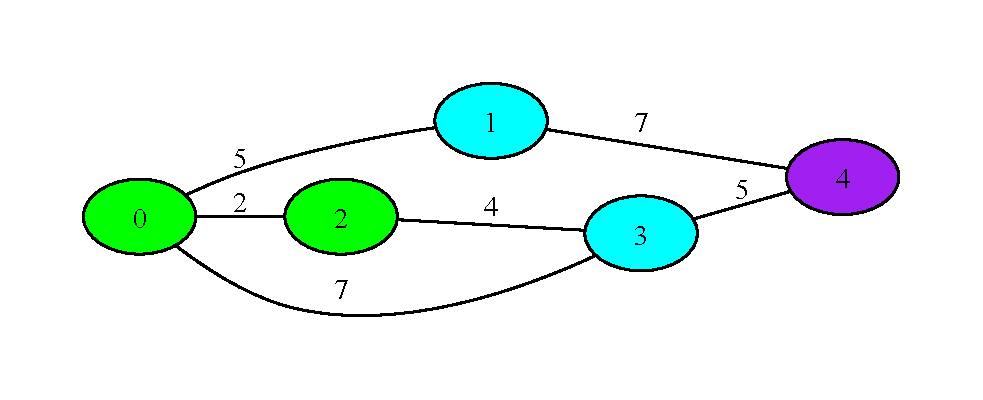
\includegraphics[scale=0.7]{figure/UCS/2.pdf}
    \caption{Ta xét cùng đồ thị hình \ref{fig:init}. Ở các bước đầu, UCS giống như BFS ở hình \ref{fig:BFS_0}, \ref{fig:BFS_1}, thế nhưng khi chọn các nút để đi tiếp sau khi mở rộng nút $0$, UCS sẽ chọn nút $2$ do $path\_cost(2) = path\_cost(0) + w(0, 2) = 2$ là nhỏ nhất trong đó $path\_cost(1) = 5$ và $path\_cost(3) = 7$.}
    \label{fig:UCS_2}
\end{figure}

\begin{figure}[H]
    \centering
    \includegraphics[scale=0.7]{figure/UCS/3.pdf}
    \caption{Tiếp theo, ta thấy $path\_cost(3) = path\_cost(2) + w(2, 3) = 2 + 4 = 6$ nhỏ hơn $path\_cost(3) = 7$ cũ nên ta thay thế $path\_cost(3)$ và chọn đi $1$ do $path\_cost(1) = 5$ là nhỏ nhất.}
    \label{fig:UCS_3}
\end{figure}

\begin{figure}[H]
    \centering
    \includegraphics[scale=0.7]{figure/UCS/4.pdf}
    \caption{Tiếp theo, ta thấy $path\_cost(4) = path\_cost(1) + w(1, 4) = 5 + 7 = 12$ lớn hơn $path\_cost(3) = 6$, do đó ta sẽ đi tiếp đến $3$.}
    \label{fig:UCS_4}
\end{figure}

\begin{figure}[H]
    \centering
    \includegraphics[scale=0.7]{figure/UCS/5.pdf}
    \caption{Cuối cùng ta sẽ có $path\_cost(4) = path\_cost(3) + w(3, 4) = 6 + 5 = 11$ bé hơn $path\_cost(4)$ cũ nên thay thế, đồng thời $frontier$ cũng còn lại duy nhất $4$, ta đi tới $4$ và đến được đích.}
    \label{fig:UCS_5}
\end{figure}

\subsection{Đánh giá}

\begin{itemize}
    \item \textbf{Tính đầy đủ}: UCS chỉ đầy đủ khi tại mọi bước trong quá trình tìm kiếm, chi phí của mỗi lần chuyển sẽ luôn lớn hơn một số dương $\epsilon$ nào đó. Giả sử lần chuyển đầu tiên có chi phí là $1/2$, lần sau là $1/4$, lần sau là $1/8$, và cứ thế, do đó không tồn tại $\epsilon > 0$ sao cho chi phí mỗi lần chuyển đều lớn hơn $\epsilon$, khi đó chi phí đường đi sẽ là $1$ cho dù phải đi qua vô hạn nút. Thế nhưng nếu chi phí đường đi tối ưu có giá trị lớn hơn $1$ thì UCS sẽ không bao giờ tìm được đáp án.

    \item \textbf{Tính tối ưu}: Như ta đã biết, nếu đồ thị không có chi phí hoặc chi phí như nhau thì UCS là BFS, do đó có tính tối ưu. Nếu đồ thị có chi phí, thì UCS sẽ tìm ra đáp án có chi phí nhỏ nhất, do đó cũng có tính tối ưu.

    \item \textbf{Độ phức tạp thời gian}: Đặt $C^*$ là chi phí đường đi tối ưu nhất, khi đó với mỗi lần chạy, chi phí đường đi sẽ gần với chi phí đương đi tối ưu thêm ít nhất một khoảng $\epsilon$ (ta dùng $\epsilon$ ở phía trên tính đầy đủ), ở khởi đầu chi phí là $0$, lần tiếp theo là $\epsilon$, tiếp theo nữa là $2\epsilon$, cho đến khi là $(C^*/\epsilon)\epsilon = C^*$, do đó độ sâu mà ta phải đi là $C^*/\epsilon + 1$. Vậy như ở trên BFS, độ phức tạp thời gian là $O(b^{C^*/\epsilon + 1})$ với $b$ là hệ số phân nhánh tiến tối đa.

    \item \textbf{Độ phức tạp không gian}: Ta biết mỗi nút đều được lưu trên bộ nhớ, do đó độ phức tạp không gian cũng giống với độ phức tạp thời gian là $O(b^{C^*/\epsilon + 1})$.
\end{itemize}

%%%%%%%%
\section{Depth-First-Search (DFS)}

\subsection{Ý tưởng chính}

DFS hay \textit{tìm kiếm theo chiều sâu} sẽ xem \textit{frontier} như một ngăn xếp, những nút được thêm vào sau sẽ được lấy ra trước, do đó DFS luôn chọn những nút sâu nhất để mở rộng (thêm càng về sau, thì nút càng sâu), ngoài ra ở DFS ta có thể bỏ tập $expanded$ đi nếu đồ thị dạng cây, lúc này bộ nhớ được sử dụng sẽ nhẹ đi. Ý tưởng của DFS là khi ta chọn 1 nút để đi, ta sẽ tiến hành đi sâu dần đường đi từ nút đó cho đến khi ta không thể đi được nữa, sau đó ta sẽ lấy nút sâu kế tiếp từ \textit{frontier} (nút phía trước nút mà ta lấy ra, nút càng về sau càng sâu như ta đã nói phía trên) để đi và cuối cùng dừng nếu gặp được trạng thái đích.

\subsection{Mã giả}

\begin{algorithm}[H]
  $start \gets \text{trạng thái bắt đầu}$\;
  \tcc{ta xem \textit{frontier} như là một ngăn xếp}
  $frontier \gets \{start\}$\; 
  $expanded \gets \emptyset$\;
  $goal \gets \text{hàm xem nút hiện tại có là trạng thái đích hay chưa}$\;
  $T \gets \text{hàm chuyển trạng thái con}$\;
  \While{$frontier \neq \emptyset$}
  {
      $current \gets \text{nút được lấy ra từ $frontier$}$\;
      \text{Thêm $current$ vào $expanded$}\;
      \eIf{$goal(current)$}
      {
        \KwRet{\text{đã tìm thấy đáp án}}\;
      }{
        \For{$neighbor \in T(current)$}
        {
            \If{$neighbor \notin frontier$ và $neighbor \notin expanded$} 
            {
                \text{Thêm $neigbor$ vào $frontier$}\;
            }
        }
      }
  }
  \KwRet{\text{không tìm thấy đáp án}}\;
  \caption{Depth-First-Search}
  \label{algo:DFS}
\end{algorithm}

\subsection{Ví dụ}

\begin{figure}[H]
    \centering
    \includegraphics[scale=0.8]{figure/DFS/2.pdf}
    \caption{Ta dùng đồ thị hình \ref{fig:init} làm ví dụ. Ở giai đoạn đầu, DFS cũng giống như BFS ở hình \ref{fig:BFS_0} và \ref{fig:BFS_1}. Thế nhưng sau khi đã mở rộng được các nút $1, 2, 3$ ta sẽ chọn nút tiếp theo bằng xem nút nào được thêm cuối cùng vào $frontier$, ta thêm lần lượt là $3, 2, 1$ (do ta ưu tiên những nút có số nhỏ hơn) và do $1$ thêm vào cuối nên ta lấy nút $1$ đầu tiên và đi tiếp.}
    \label{fig:DFS_2}
\end{figure}

\begin{figure}[H]
    \centering
    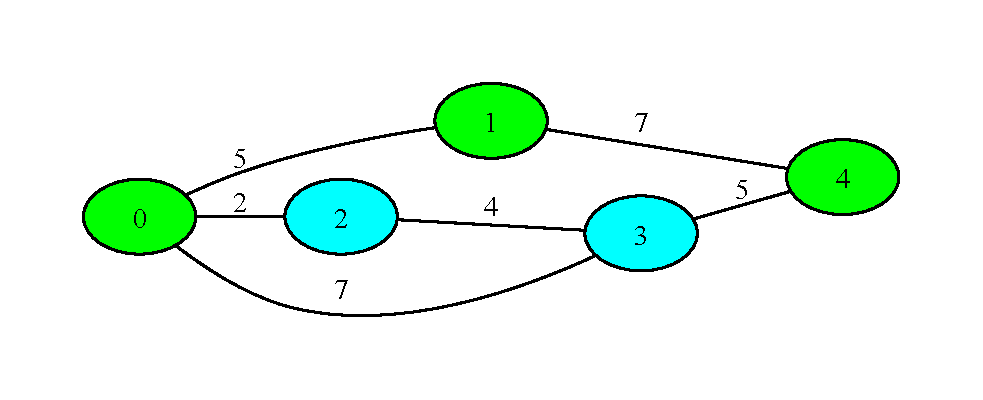
\includegraphics[scale=0.8]{figure/DFS/3.pdf}
    \caption{Sau khi đã chọn mở rộng nút $1$, ta tìm được nút $4$ và đưa nút $4$ và $frontier$, do $4$ được đưa vào cuối cùng nên ta lấy $4$ ra đầu tiên và đi tới $4$, đồng thời ta cũng tìm được trạng thái đích.}
    \label{fig:DFS_3}
\end{figure}

\subsection{Đánh giá}

\begin{itemize}
    \item \textbf{Tính đầy đủ}: Trên một đồ thị dạng cây hữu hạn thì DFS luôn đảm bảo tìm được đáp án, thế nhưng ở đồ thị vô hạn, nó sẽ đi liên tục trên một đường đi vô hạn. Trên các đồ thị có hướng không chu trình (\textit{acyclic directed graph}) nếu ta không có tập $expanded$, DFS có thể mở rộng một nút nhiều lần thông qua các đường đi khác nhau, nếu may mắn nút có hệ số phân nhánh lùi thấp, ta vẫn có thể đảm bảo được việc tìm ra đáp án trong hữu hạn thời gian. Trong các đồ thị có chu trình (\textit{cyclic graph}), nếu ta không có tập $expanded$ thì DFS sẽ đi vòng lại, dẫn đến bị kẹt trong một vòng lặp vô hạn \cite{Russell_Norvig_Chang_2022}. Do đó DFS không đảm bảo được tính đầy đủ.

    \item \textbf{Tính tối ưu}: DFS không đảm bảo được tính tối ưu, do đáp án mà nó trả về là đáp án đầu tiên mà nó tìm thấy, tức là DFS sẽ chọn một đường đi khả thi và đi cho đến khi tìm được đáp án rồi trả về đáp án. Đường đi mà DFS chọn có thể không tối ưu hoặc có thể là tồi nhất.

    \item \textbf{Độ phức tạp thời gian}: Xét trên một đồ thị hữu hạn và ta có tập $expanded$. Giả sử trạng thái đích ở độ sâu $m$ và mỗi nút có hệ số phân nhánh tiến tối đa là $b$. Trong trường hợp xấu nhất DFS phải đi hết toàn bộ đồ thị, khi nó không chọn đúng đường đi và phải đi lại, do đó mất $O(b^m)$, riêng trường hợp tốt nhất, DFS chỉ cần đi đúng một đường đi dẫn đến kết quả và mất $O(m)$.

    \item \textbf{Độ phức tạp không gian}: DFS chỉ lưu những nút mà trên đường đi nó chọn, giả sử trạng thái đích nằm ở độ sâu $m$ và hệ số phân nhánh tiến tối đa là $b$, khi đó DFS chỉ cần lưu $b \cdot m + 1$ nút. Nếu ta thêm tập $expanded$ thì phải lưu thêm tối đa $m$ nút, do đó sẽ lưu $b\cdot m + 1 + m = (b + 1)\cdot m +1$ nút, vậy độ phức tạp không gian vẫn sẽ là $O(b\cdot m)$.
\end{itemize}

%%%%%%
\newpage
\section{$\text{A}^*$ Search}

\subsection{Ý tưởng chính}

Tìm kiếm $\text{A}^*$ là một trong những thuật toán tìm kiếm nổi bật của tìm kiếm có thông tin. Giống như UCS, $\text{A}^*$ cũng xem $frontier$ như một \textit{hàng đợi ưu tiên} nhưng trong đó ta sẽ ưu tiên theo hàm $f(n)$ được tính như sau:
$$
f(n) = path\_cost(n) + h(n)
$$
với $path\_cost(n)$ là chi phí đường đi từ nút đầu tiên đến $n$ và $h(n)$ là hàm heuristic tại nút $n$. Trong đó $\text{A}^*$ sẽ chọn những nút có $f(n)$ nhỏ nhất, ta biết $f(n)$ nhỏ nhất khi $g(n)$ và $h(n)$ nhỏ nhất, do đó việc này đảm bảo tìm được chi phí đường đi tối ưu đồng thời cũng gần trạng thái đích do càng gần trạng thái đích thì $h(n)$ càng nhỏ. Vì vậy việc quan trọng nhất là ta phải chọn được $h(n)$ sao cho $\text{A}^*$ là tốt nhất, nếu ta chọn $h(n)$ tồi thì đôi khi $\text{A}^*$ còn tệ hơn UCS.
\vspace{7pt}

Ngoài ra, có những bài toán có ``dạng'' cụ thể để ta có thể chọn được hàm $h(n)$ tốt nhất, ví dụ bài toán tìm đường đi giữa hai thành phố thì ta có thể đặt $h(n)$ là khoảng cách nối giữa hai thành phố đó (độ dài đường thẳng nối hai thành phố), nếu bài toán chúng ta được thực hiện trên một mặt hai chiều chia thành từng ô vuông nhỏ (ví dụ pixel màn hình máy tính) thì ta có thể chọn $h(n)$ là \textit{khoảng cách Manhattan} hoặc \textit{khoảng cách Chebyshev}.

\subsection{Mã giả}

\begin{algorithm}[H]
  $start \gets \text{trạng thái bắt đầu}$\;
  \tcc{ta xem \textit{frontier} như là một hàng đợi ưu tiên}
  \tcc{ta sẽ thêm nút $n$ cùng với $f(n)$ vào $frontier$}
  \tcc{ta sẽ ưu tiên những nút có $f(n)$ nhỏ lên phía trước}
  \tcc{do $start$ là nút đầu tiên nên $f(start) = path\_cost(start) + h(start) = 0 + h(start) = h(start)$}
  $frontier \gets \{\{h(start), start\}\}$\; 
  $expanded \gets \emptyset$\;
  $goal \gets \text{hàm xem nút hiện tại có là trạng thái đích hay chưa}$\;
  $T \gets \text{hàm chuyển trạng thái con}$\;
  \tcc{$path\_cost(n)$ sẽ trả về chi phí đường đi từ trạng thái ban đầu đến nút $n$}
  $path\_cost \gets \text{hàm trả về chi phí đường đi tối ưu}$\;
  \tcc{$w(n',n)$ sẽ trả về trọng số của cạnh $n'n$}
  $w \gets \text{hàm lấy trọng số của một cạnh}$\;
  \While{$frontier \neq \emptyset$}
  {
      $current \gets \text{nút được lấy ra từ $frontier$}$\;
      \text{Thêm $current$ vào $expanded$}\;
      \eIf{$goal(current)$}
      {
        \KwRet{\text{đã tìm thấy đáp án}}\;
      }{
        \For{$neighbor \in T(current)$}
        {
            $neighbor\_cost \gets path\_cost(current) + w(current, neighbor)$\;
            \uIf{$neighbor \notin frontier$ và $neighbor \notin expanded$}
            {
                \tcc{Khác với UCS, ta sẽ ưu tiên lấy nút từ $frontier$ dựa vào $f = path\_cost + h$}
                $f \gets neighbor\_cost + h(neighbor)$\;
                \text{Thêm $\{f, neighbor\}$ vào $frontier$}\;
            }
            \uElseIf{$neighbor \in frontier$ và $neighbor\_cost < path\_cost(neighbor)$}
            {
                \tcc{Cũng giống như UCS, nếu ta tìm được đường đi có $path\_cost$ tốt hơn, ta sẽ thay thế $path\_cost$ cũ}
                $path\_cost(neighbor) \gets neighbor\_cost$\;
            }
        }
      }
  }
  \KwRet{\text{không tìm thấy đáp án}}\;
  \caption{$\text{A}^*$ Search}
  \label{algo:AStar}
\end{algorithm}

\newpage
\subsection{Ví dụ}

\begin{figure}[H]
    \centering
    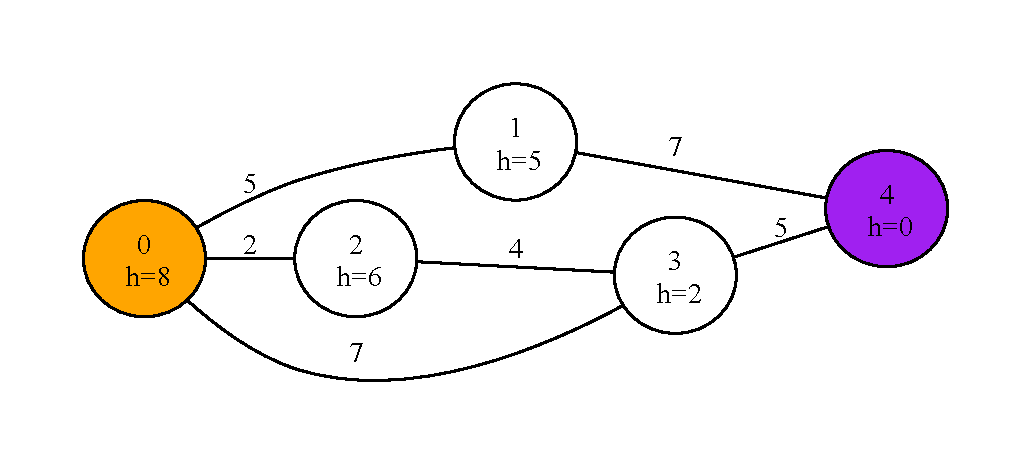
\includegraphics[scale=0.7]{figure/init_heuristic.pdf}
    \caption{Ta sẽ dùng lại đồ thị ở hình \ref{fig:init} thế nhưng ta sẽ thêm $heuristic$ cho từng nút (được kí hiệu là $h=$).}
    \label{fig:init_heu}
\end{figure}

\begin{figure}[H]
    \centering
    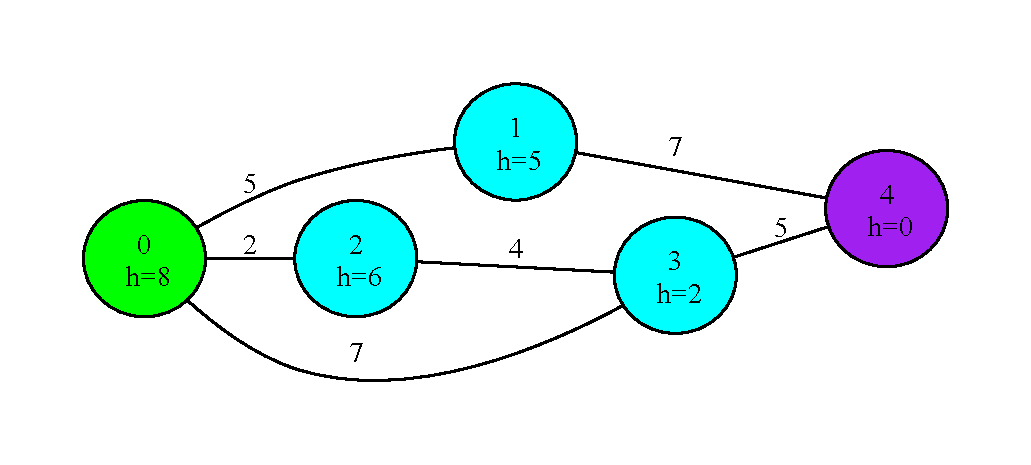
\includegraphics[scale=0.7]{figure/AStar/1.pdf}
    \caption{Ở giai đoạn đầu, $\text{A}^*$ sẽ chọn mở rộng nút $0$ do chỉ có mỗi nút $0$ trong $frontier$, sau mở rộng được nút $1,2,3$. Về cơ bản thì giai đoạn này cũng gần giống với các thuật toán trên.}
    \label{fig:AStar_1}
\end{figure}

\begin{figure}[H]
    \centering
    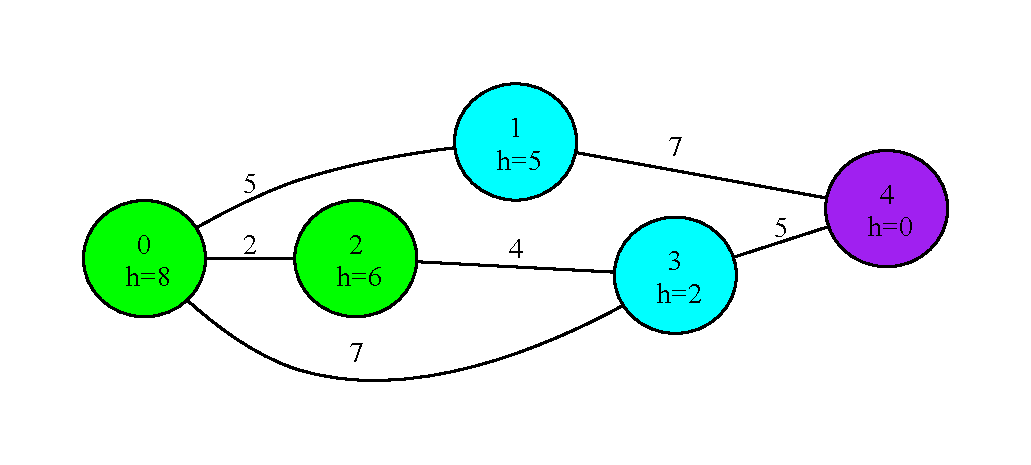
\includegraphics[scale=0.7]{figure/AStar/2.pdf}
    \caption{Ở giai đoạn tiếp theo, ta có $f(2) = path\_cost(2) + h(2) = 2 + 6 = 8, f(1) = 5 + 5 = 10$ và $f(3) = 7 + 2 = 9$. Do nút $2$ có giá trị $f$ nhỏ nhất nên ta sẽ ưu tiên đi đến $2$ và mở rộng được $3$.}
    \label{fig:AStar_2}
\end{figure}

\begin{figure}[H]
    \centering
    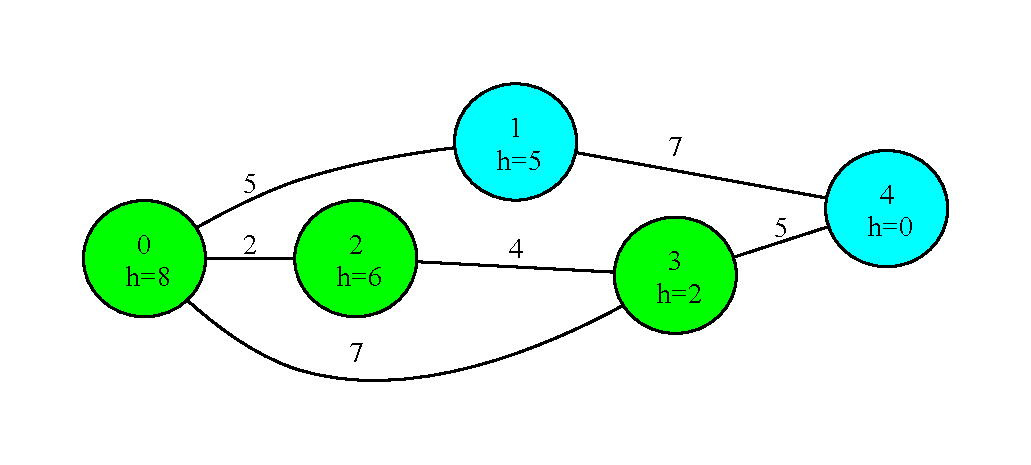
\includegraphics[scale=0.7]{figure/AStar/3.pdf}
    \caption{Tiếp theo, $path\_cost(3)$ thông qua đường đi $2$ sẽ là $6$ so với $7$ nếu đi qua $0$, do đó ta thay thế $path\_cost(3) = 6$. Tiếp theo $f(3) = path\_cost(3) + h(3) = 6 + 2 = 8$ vẫn bé hơn $f(1) = 10$ nên ta sẽ chọn đi tiếp đến $3$ và mở rộng được nút $4$.}
    \label{fig:AStar_3}
\end{figure}

\begin{figure}[H]
    \centering
    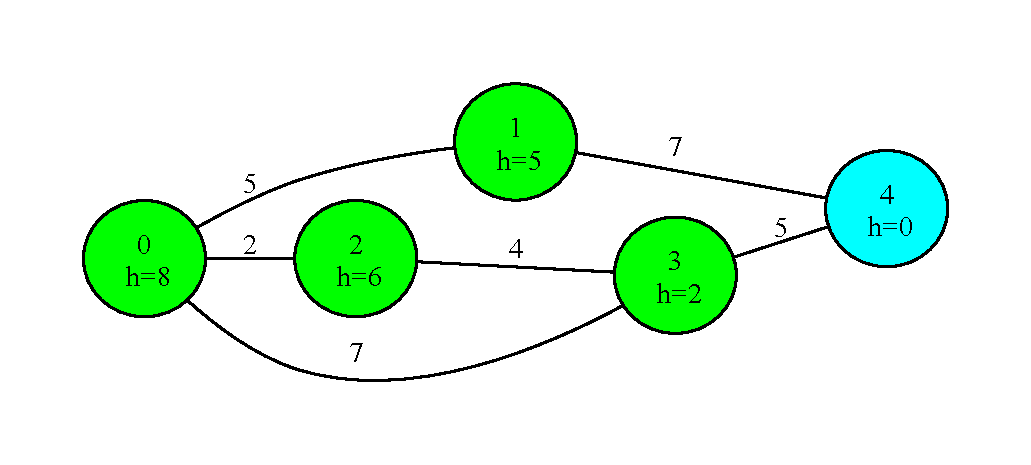
\includegraphics[scale=0.7]{figure/AStar/4.pdf}
    \caption{Tiếp theo, $3$ đã mở rộng được nút $4$, ta có $path\_cost(4) = path\_cost(3) + 5 = 11$ do đó $f(4) = 11 + h(4) = 11$ lớn hơn so với $f(1)$ nên ta sẽ chọn đi đến $1$ thay vì $4$.}
    \label{fig:AStar_4}
\end{figure}

\begin{figure}[H]
    \centering
    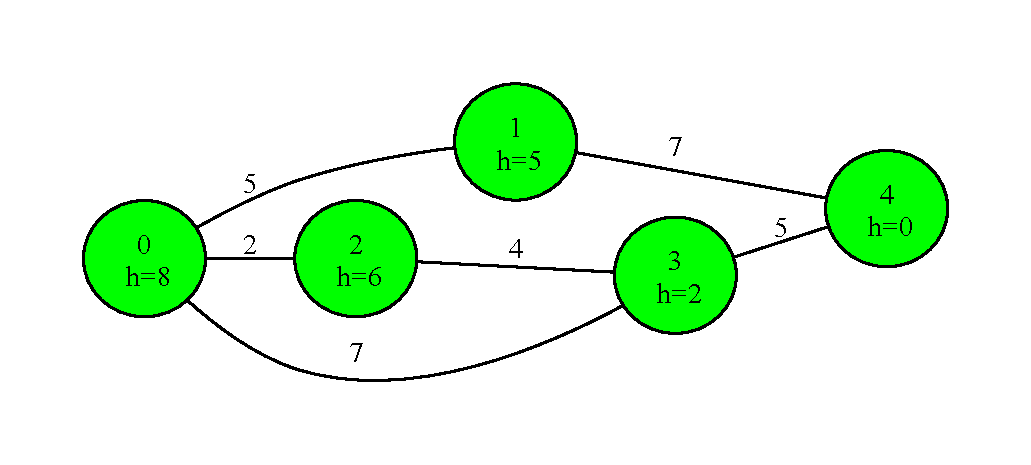
\includegraphics[scale=0.7]{figure/AStar/5.pdf}
    \caption{Cuối cùng, đi đến $1$ ta mở rộng được $4$ và $path\_cost(4)$ mới sẽ là $path\_cost(1) + 7 = 12$ do đó lớn hơn $path\_cost(4)$ cũ là $11$, nên ta sẽ chọn đi tới $4$ thông qua $3$. Và như vậy ta đã đến được trạng thái đích.}
    \label{fig:AStar_5}
\end{figure}

\newpage
\subsection{Đánh giá}
\begin{itemize}
    \item \textbf{Tính đầy đủ}: Như UCS, nếu chi phí của mỗi lần chuyển luôn lớn hơn một số dương $\epsilon$ nào đó, khi đó $A^*$ có tính đầy đủ.
    
    \item \textbf{Tính tối ưu}: $\text{A}^*$ có tính tối ưu hay không sẽ phụ thuộc vào hàm heuristic ta chọn có chấp nhận được hay không. Vì vậy ta chỉ cần chọn được hàm heuristic chấp nhận được, $\text{A}^*$ sẽ tối ưu. 
    \begin{proofvn}
        Ta dùng chứng minh phản chứng. Giả sử hàm heuristic chấp nhận được nhưng $\text{A}^*$ chưa tối ưu, khi đó chi phí đường đi mà đáp án $\text{A}^*$ trả về (gọi là $p$) sẽ có chi phí cao hơn đường đi có chi phí tối ưu thật sự (gọi là $p'$), đặt chi phí tối ưu thật sự là $C^*$. Đường đi $p$ sẽ gồm $start \rightarrow goal$ và đường đi $p'$ sẽ gồm $start \rightarrow s$ (bởi vì khi có được $p$, $\text{A}^*$ sẽ dừng, do đó $p'$ sẽ dừng tại nút $s$ nào đó mà chưa đi được đến $goal$). Vì vậy, tại bước cuối cùng, $frontier$ sẽ chọn $goal$ thay vì nút $s$, do đó:
        \begin{align*}
        f(goal) &\leq f(s) \\
        \implies path\_cost(goal) + h(goal) &\leq path\_cost(s) + h(s) \\
        \implies path\_cost(goal) &\leq path\_cost(s) + h(s) \\
        \implies path\_cost(goal) &\leq path\_cost(s) + h^*(s) \hspace{5pt} \text{($h$ chấp nhận được)} \\
        \implies path\_cost(goal) &\leq C^*
        \end{align*}
        Điều trên sai với giả sử ban đầu (nghĩa là $path\_cost(goal) > C^*$), thế nên $A^*$ sẽ tối ưu khi mà hàm heuristic $h$ chấp nhận được.
    \end{proofvn}
    Thế nhưng ngược lại, $\text{A}^*$ vẫn có thể tối ưu nếu hàm heuristic không chấp nhận được. Ngoài ra nếu ta chọn được hàm heuristic nhất quán thì $\text{A}^*$ luôn có tính tối ưu.
    
    \item \textbf{Độ phức tạp thời gian}: Trong trường hợp xấu nhất, $\text{A}^*$ phải tìm kiếm toàn bộ không gian trạng thái, do đó nếu hệ số phân nhánh tiến tối đa là $b$, độ sâu tối đa là $m$ thì độ phức tạp sẽ là $O(b^m)$.
    
    \item \textbf{Độ phức tạp không gian}: Cũng giống như các thuật toán trên, mỗi nút sinh ra đều được lưu trên bộ nhớ, do đó độ phức tạp không gian trong trường hợp xấu nhất cũng giống với độ phức tạp thời gian là $O(b^m)$.
\end{itemize}

%%%%%%%%
\section{Greedy Best-First-Search}

\subsection{Ý tưởng chính}

Khác đi một chút so với $\text{A}^*$ và UCS, Greedy cũng xem $frontier$ như hàng đợi ưu tiên nhưng sẽ ưu tiên những node có heuristic (thay vì chi phí đường đi như UCS hay hàm $f$ như $\text{A}^*$) tốt hơn (tức là thấp hơn). Do đó ta có thể nói Greedy là \textit{tối ưu cục bộ} do tại một bước bất kì nào đó, Greedy luôn tối ưu, tìm được nút có giá trị heuristic tốt nhất.

\newpage
\subsection{Mã giả}

\begin{algorithm}[H]
  $start \gets \text{trạng thái bắt đầu}$\;
  \tcc{ta xem \textit{frontier} như là một hàng đợi ưu tiên}
  \tcc{những nút có heuristic càng tốt (thấp hơn) sẽ được ưu tiên lên đầu}
  $frontier \gets \{\{h(start), start\}\}$\; 
  $expanded \gets \emptyset$\;
  $goal \gets \text{hàm xem nút hiện tại có là trạng thái đích hay chưa}$\;
  $T \gets \text{hàm chuyển trạng thái con}$\;
  \While{$frontier \neq \emptyset$}
  {
      $current \gets \text{nút được lấy ra từ $frontier$}$\;
      \text{Thêm $current$ vào $expanded$}\;
      \eIf{$goal(current)$}
      {
        \KwRet{\text{đã tìm thấy đáp án}}\;
      }{
        \For{$neighbor \in T(current)$}
        {
            \If{$neighbor \notin frontier$ và $neighbor \notin expanded$} 
            {
                \text{Thêm $\{h(neighbor), neigbor\}$ vào $frontier$}\;
            }
        }
      }
  }
  \KwRet{\text{không tìm thấy đáp án}}\;
  \caption{Greedy Best-First-Search}
  \label{algo:Greedy}
\end{algorithm}

\subsection{Ví dụ}

\begin{figure}[H]
    \centering
    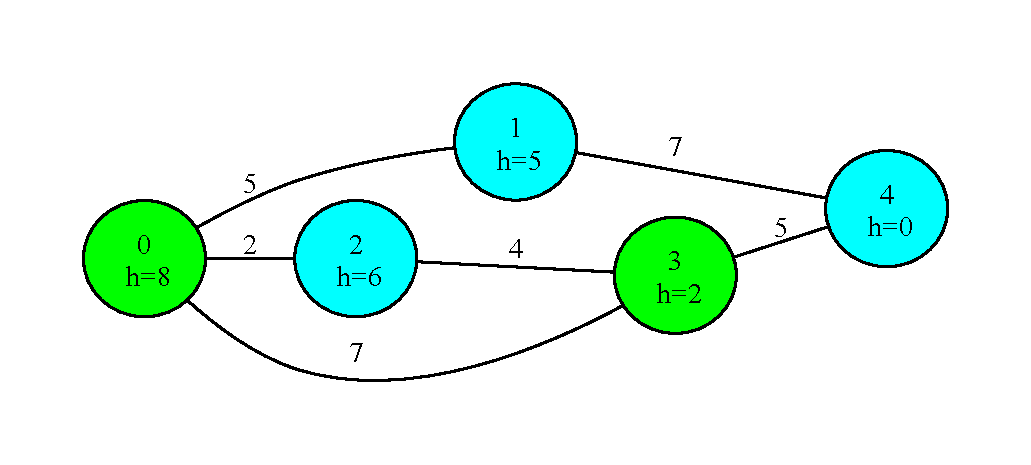
\includegraphics[scale=0.7]{figure/Greedy/2.pdf}
    \caption{Ta sẽ dùng lại hình \ref{fig:init_heu} làm ví dụ. Ở các bước ban đầu, Greedy cũng tương tự như các thuật toán trên, để chọn giữa các nút được mở rộng $1, 2, 3$, Greedy sẽ chọn nút có heuristic thấp nhất, do đó nút $3$ với $h=2$ sẽ được chọn để đi tiếp.}
    \label{fig:Greedy_2}
\end{figure}

\begin{figure}[H]
    \centering
    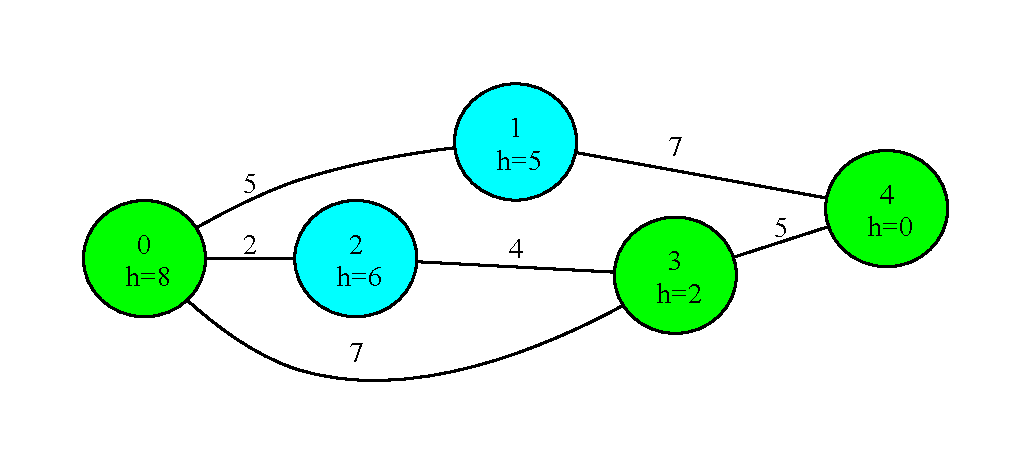
\includegraphics[scale=0.7]{figure/Greedy/3.pdf}
    \caption{Ở bước cuối cùng, sau khi chọn mở rộng $3$, ta tìm được nút $4$ với $h=0$, đồng thời cũng là tốt nhất nên ta chọn đi đến $4$, ngoài ra $4$ cũng là trạng thái đích nên Greedy dừng.}
    \label{fig:Greedy_3}
\end{figure}

\subsection{Đánh giá}

\begin{itemize}
    \item \textbf{Tính đầy đủ}: Greedy luôn có tính đầy đủ trên một đồ thị hữu hạn. Giả sử nếu các nút có heuristic là như nhau, thì Greedy tương tự như BFS.

    \item \textbf{Tính tối ưu}: Ta thấy Greedy chỉ chọn những nút có heuristic tốt nhất nên sẽ phụ thuộc nhiều vào heuristic, Greedy không quan tâm đến các chi phí đường đi, do đó đường đi mà Greedy tìm ra sẽ có thể không có chi phí tối ưu. Thế nên Greedy không đảm bảo tính tối ưu.

    \item \textbf{Độ phức tạp thời gian}: Trong trường hợp xấu nhất, Greedy phải tìm kiếm hết không gian trạng thái, nếu mỗi nút có hệ số phân nhánh tiến là $b$ và độ sâu tối đa của không gian trạng thái là $m$ thì độ phức tạp thời gian là $O(b^m)$.

    \item \textbf{Độ phức tạp không gian}: Giống như DFS, khi hết đường Greedy phải quay lui về để tìm các đường đi khác. Thế nhưng, ở DFS khi ta chỉ quay lui về các nút con của những nút cha đã được mở rộng, thì Greedy lại quay lui về ngẫu nhiên về các nút khác trong đồ thị và mở rộng các nút đó, lúc mở rộng ta phải lưu lại các nút đó (cùng heuristic của nó) để dùng sau này, nên trường hợp xấu nhất là ta phải lưu hết tất cả các nút, do đó độ phức tạp là $O(b^m)$.
\end{itemize}